\chapter{Related Work}

In the following section we want to investigate the current state of research on 6D pose estimation to get a hold of the state-of-the-art methods in this field. For the sake of a smooth entrance, but also to enable the reader to put the efforts of today into perspective, the chapter starts with an excerpt of hand-crafted methods. We then proceed to present the latest papers in this field and last but not least analyze publications on active learning and fine-tuning of neural networks, as this is also part of this work.

\section{Research on 6D Pose Estimation}

Pose estimation has become an interesting problem with the advent of robots in production, as well as the relatively new area of virtual and augmented reality \cite{bb8}. Former research focused on manual feature extraction, divided into the major groups of sparse and dense approaches, as well as template-based ones. Nowadays scientists of course often employ learning-based techniques which offer better and better results.

\subsection{Non-Learning-Based}

Before the major breakthrough of deep learning in 2012, handcrafted feature-based approaches were common for 6D pose estimation \cite{ylecun}. A lot of research \cite{gklein,dglowe2,charris} made use of edges to detect 3D objects, but were therefore sensitive to occlusion for example. Methods relying on keypoints \cite{dglowe1, dwagner} worked well on well-textured objects and were popular for some time. But as already implied, they yielded bad performance on poor-textured or texture-less objects, obviously due to the inferior quality or complete absence of the keypoints. 

An intuitive idea, to improve the quality of the estimate, is to use stereo cameras, as in \cite{kpauwels}. A second image from another angle provides additional information. But this simply shifted the problem towards stereo-matching, which, to the day, remains a complex task. The sudden availability of cheap depth sensors, like the Kinect, gave rise to algorithms making use of RGB-D images since it was now easy to setup a cheap system that provided depth information of suitable grade. Different approaches are possible when incorporating depth to retrieve an object's pose. \cite{bdrost, salasmoreno} developed systems that achieved good results by voting of pairs of 3D points of objects and their respective normals. In contrast to edge detection, occlusion can be handled better this way and does not corrupt the result. 

Template-based methods \cite{hinterstoisser1, hinterstoisser2, rioscabrera, csteger} use generated views of the object at different angles which are then slid over the image as a scanner  for tracking and detection and offer good performance on texture-less or poor-textured objects. 

\subsection{Learning-Based}

As mentioned earlier, the feature- and template-based approaches once were the first choice, but methods that learn a part of the information of the objects - that is not explicitly modeled - started to outperform the previous techniques.

\cite{klai} uses decision tress which incorporate the semantic information of objects and their poses. Here, the researchers moved from manually modeling features to actual learning. \cite{dtome} predicts human poses from single RGB images in an end-to-end fashion. The authors incorporate a prior over the poses and show how predicting landmarks can be part of the CNN itself so that the method does not have to be setup in a pipelined fashion. And \cite{azeng} relies on multi-view images and depth information and was able to develop a system that scored the 3rd and 4th place in the Amazon Picking Challenge 2016. There exists a vast literature on learned pose estimation but unfortunately due to time-constraints only a selection can be discussed here.

\quad \textbf{BB8}

BB8 \cite{bb8}, which is an abbreviation for the 8 corners of the bounding-boxes of objects, is the only recently developed method by Rad and Lepetit that works on RGB-only images. Instead of regressing the pose of an object with object coordinates like \cite{brachmann1}, they let a deep neural network estimate the object segmentations first and then predict the 2D locations of the 3D corners of the bounding box. 

\begin{figure}[!tbp]
	\centering
	\begin{subfigure}[b]{0.45\textwidth}
		\centering
    	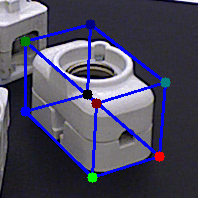
\includegraphics[width=0.45\linewidth]{bb8}
    	\caption{The control points of the object's bounding box. \cite{bb8}}
	\end{subfigure}
	\hfill
	\begin{subfigure}[b]{0.45\textwidth}
		\centering
    	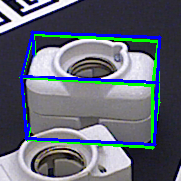
\includegraphics[width=0.45\linewidth]{bb8_prediction}
    	\caption{The final estimated pose. Green is the groundtruth. \cite{bb8}}
	\end{subfigure}
	\caption{Example images displaying the functioning of BB8. \cite{bb8}}
\end{figure}

Despite its differences to \cite{brachmann1}, the object's position is not predicted directly either but instead regressed by solving the perspective-n-point problem implied by the output of the network. The architecture of the first and second net is based on VGG respectively but with the last layer cut off and replaced by a fully connected on which is adjusted to the problem by fine-tuning it. 

The first network, which segments the image, helps estimating the pose of the object in a way that the second network positions its window at the center of the segmentation. This also makes it clear that the approach reasons globally about the pose and does not learn only patches of the object that is to be detected. The authors argue that the patch-based pose estimators are typically very noisy, and hence require a robust optimization scheme, like e.g. RANSAC. 

Unfortunately, BB8's take on pose estimation fails on symmetric objects when implemented directly as described above. As a result, the authors introduce a novel system that takes into account an axis of symmetry of objects. Since the object's rotation around it's axis of symmetry can be defined by modulo its angle of symmetry but the pose predictions around 0 and the angle itself can still be pretty bad, the authors divided the rotational range in two halves and restricted the training of the network to the first half. An additional CNN classifier, which is run before the actual estimator, predicts whether the object's current angle of rotation is within the first or second half, and in the latter case mirrors the image. This way, the CNN only trained on one half of the rotational range can still be applied. For objects that are not exactly symmetrical they divide the range into four parts and pre-predict whether the object's rotation is within the first or second quarter. 

The proposed method offers good performance and can compete and surpass state-of-the-art research. Given the temporal frame of this work which allows only for the fundamental exploration of a narrow set of methods, the likewise good performance of \cite{brachmann2} and \cite{pertsch}, and the assumption of the author that, due to the often only patch-wise visibly instruments which calls for a non-global reasoning design, \cite{bb8} might not be as performant, this approach is not further investigated or incorporated into this work.

\quad \textbf{SSD-6D}

The system carved out by \cite{ssd-6d} is based on the work by \cite{ssd} dubbed Single-Shot Multibox Detector, or short SSD. Their take on 6D pose estimation is especially alluring, as the authors train the network exclusively on synthetic data. Good results would imply that the lack of large already annotated datasets for 6D pose estimation in the field of biomedical imaging could be overcome by simply generating the desired amount of data and training the network on this artificial data. 

In contrast to BB8 and Brachmann et al., who both rather inferred what part of the image corresponds to what of the object to be detected, Kehl et al. let the network estimate the probability of a discrete viewpoint, which is essentially a view of a camera on the object. Those viewpoints are sampled equidistant alongside a degree step-size to represent all possible poses of the objects. According to the authors, the number of views that are necessary to produce good results is 642. In addition, in-plane rotations of the objects are sampled as well. This view estimate combined with an estimate on the rotation is used to generate pose predictions. 

\begin{figure}[!tbp]
	\centering
	\begin{subfigure}[b]{0.5\textwidth}
		\centering
    	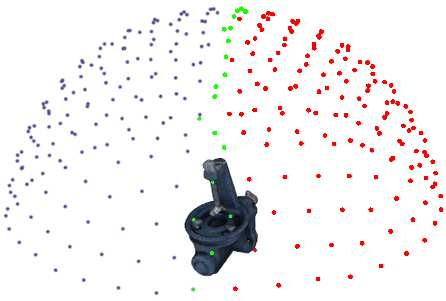
\includegraphics[width=0.5\linewidth]{ssd_6d_sphere}
    	\caption{An exampe of a discrete distribution of viewpoints on an object. \cite{ssd-6d}}
	\end{subfigure}
	\hfill
	\begin{subfigure}[b]{0.4\textwidth}
		\centering
    	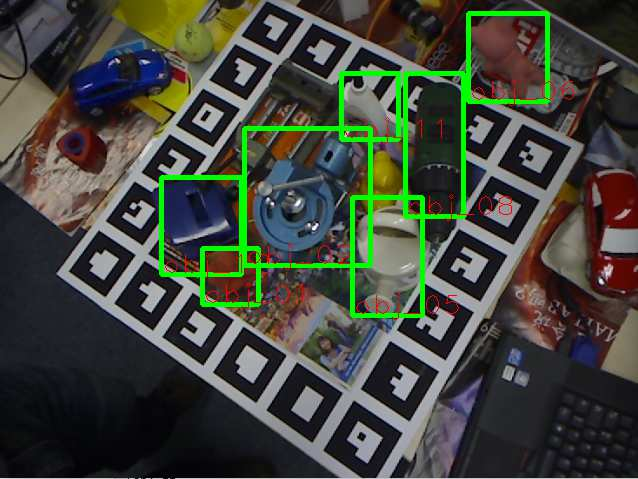
\includegraphics[width=0.5\linewidth]{ssd_6d_bb}
    	\caption{Left images: An example for bounding boxes found by the SSD-6D network. Right images: The most confident views and rotations for those boxes.  \cite{ssd-6d}}
	\end{subfigure}
	\caption{Example images displaying the functioning of SSD-6D. \cite{ssd-6d}}
\end{figure}

The network architecture, that is inspired by SSD, produces feature maps using branches from a pre-trained Inception V4, which was introduced in \cite{inceptionv4}. The branches are kernels of different size and the resulting maps are again convolved with kernels that predict the object class, 2D bounding box, viewpoint scores and in-plane rotations. A non-max suppression then selects only the strongest candidates. The network is trained entirely on images from the MS COCO dataset \cite{mscoco} that the authors rendered the objects into with random transformations, i.e. the whole training set is generated. For each transformation, the network is given the closest discrete viewpoint, in-plane rotation and the tightest bounding box as a regression target. As an optimization target during error-back propagation, the authors employ a loss similar to the one of SSD \cite{ssd} or YOLO \cite{yolo}. 

Like stated above, the actual 6D pose estimation task is solved by using the viewpoint, the bounding box and the in-plane rotation. The author's reasoning, that their approach on pose estimation is a more natural one than pose regression makes sense, as for example a human being rather learns what an object looks like from different angles than regression of object coordinates. Nevertheless, the network produces rather bad results if not the last step of optimization is applied. That is, after obtaining an initial pose from the network, an optimization scheme extracts 3D contour points from the rendered hypothesis, which are then used to find the closest edges to minimize a projection error and improve the overall pose. 

What can be easily verified is that the first estimate of the 6D pose is rather bad. Compared with other works, which directly produce good results with the method as is, here the most important part seems to be the second optimization program. But then, this optimization could also be used in \cite{brachmann2} or \cite{bb8} as a last step, making it a good contribution but as an addition. Thus the network architecture isn't considered any further.

\quad \textbf{Kurmann et al.}

Despite the obvious field for 6D pose estimation being autonomous robots interacting with their environment, there exists work that directly work on pose estimation of surgical instruments in minimally invasive surgery, for example \cite{kurmann}. The authors of that paper argue that the common two-stage pipeline for 6D pose estimation, that consists of object detection and then the actual pose estimation, is rather sensitive to parameter-tuning and results in a more complicated design. They also criticize that a sliding window approach might miss very small or very large instruments. 

Similarly to object coordinate regression, Kurmann et al. develop a system that produces probabilities of the presence of an object but not in a dense way but instead only for the joints of the tools. Their design draws on a scene model which holds how many tools can be visible at most, what tools are currently visible and what parts of those tools. 

The architecture of the employed network is based on the U-Net of \cite{oronneberger} and trained by optimizing the cross-entropy derived from the scene model described earlier. To adapt the architecture of U-Net, which stems from semantic segmentation, a new fully-connected layer, which is directly connected with the first layer of the network, is introduced and trained to predict probabilities of the different instruments. 

The results of the design look promising and runtimes per image are around $100 ms$, enabling it to be deployed as a near-realtime solution. On the other hand it seems like mainly literature of the biomedical imaging was considered and compared, i.e. overlooking the vast literature on 6D pose estimation in other fields. This and because object coordinates is a well-researched approach, the latter was chosen as a basis for this work over the one in \cite{kurmann}. 

\subsection{Learning-Based: Object Coordinate Regression}

An interesting section of learning-based pose estimation are the works employing the method of so-called object coordinate regression. Further information can be found in Section \ref{objectcoordinates}. The idea is based on \cite{tsharp}, who used object coordinates before. 

\cite{brachmann1} achieved record-breaking results on 6D pose estimation for texture-less objects and good performance in general and thus spawned more research in this direction. Brachmann et al. based their work not on trees but whole forests instead to regress the object's pose. The forests are trained to jointly predict the probability of object instances as well as the object coordinate probability for a given pixel, i.e. the leaves represent probability distributions. The energy function that processes the output of the forest imposes an energy minimization problem to regress the object's pose. To improve the resulting pose and make the design more robust to outliers, a RANSAC-like scheme is proposed that iteratively samples pose hypotheses and finally outputs the pose with the lowest energy.

In \cite{brachmann2}, Brachmann et al. adjusted their pipeline from \cite{brachmann1} to work with RGB-only images. To reduce uncertainty in the object instance and coordinate predictions they incorporate a self-developed auto-context framework and also marginalize the object coordinates over the depth information to cope with the missing fourth channel. The proposed system outperforms Brachmann's previous work but still relies on decision trees. \cite{akrull} elaborated \cite{brachmann1} by replacing the energy function by a CNN. This way they were able to further improve the performance of the already powerful system. Although \cite{trees-vs-cnn} finds, that random forests partly offer a slightly superior performance, their accuracy can still be comparable and we are still only on the verge of what is possible with neural networks.

\quad \textbf{Pertsch}

Although \cite{pertsch} also works with RGB-D images, we present his work here as the author proposes an easy extension to adapt the entire process to RGB-only images and presents promising results. The work by Pertsch is based on \cite{brachmann1}, i.e. likewise uses object coordinates  (see section \ref{objectcoordinates}), but replaces the random forest with a CNN. The developed pose estimation pipeline relies on three steps. The first one segments the image, the second regresses the object coordinates, and the last one evaluates pose hypotheses. 

We don't to go into detail into the first operation of the pipeline as our training and test data already includes segmentations and we can hence omit it completely. The purpose of the segmentation masks produced in the first step is to crop the area that the CNN of the second stage has to evaluate and also to calculate the score of a pose hypothesis in the energy function of the last stage. 

The second stage, which is more interesting for us, uses a multilayer CNN-architecture to predict the object coordinates. The architecture resembles an encoder-decoder network with fully-connected layers in the middle. This supposedly enables the network to detect features of the input images on a global scale as the perceptive fields of the fully-connected neurons is effectively enlarged to the full input dimensions, whereas a fully-convolutional network might miss certain connections. 

Inspired by \cite{oronneberger}, the author assimilates skip-layer connections. The network computes object coordinates for each pixel of the cropped image. To train the network the groundtruth is computed by rendering the model of the 3D object using the manually annotated groundtruth pose. Since the prediction of the object coordinates is typically quite noisy \cite{bb8}, \cite{pertsch} employs a RANSAC-scheme to improve the quality of the predicted final pose. Two different methods to retrieve the pose are presented in the work, one relying on the energy function introduced in \cite{brachmann1} but in an altered version taking into account the binary segmentation mask opposed to the random forest probabilities, and one procedure solely drawing on RGB information without the additional groundtruth depth of a sensor. The latter, which is more relevant for us as we do not have any depth readings, is based on the earlier presented \cite{brachmann2}. 

Instead of penalizing depth divergences, the number of pixels whose reprojection error is greater than a certain threshold is minimized iteratively by the RANSAC algorithm. This allows for the RGB-only extension that the author proposes but does not elaborate any further beyond a short passage. The fourth dimension is discarded by substituting the Kabsch algorithm that regresses a set of 3D-3D point pairs with a Perspective-n-Point (PnP) solver, which takes at least four 3D-2D point correspondences as input and calculates the implied pose. The 3D reprojection error is replaced by the 2D reprojection error, due to the lack of a groundtruth point cloud. We pursue a similar approach in our work which differs in architecture in the network, the steps of the pipeline (i.e. only object coordinate prediction and pose estimation) and the input data. But the general ideas of \cite{pertsch} and especially \cite{brachmann1} are adopted and further complemented with current research and active and incremental learning.

\section{Research on Active and Online Learning}

There exists a lot of research on active learning which has been conducted in the recent years. \cite{activesurvey} gives an overview over methods developed before 2011. \cite{dwang} might be among the first to incorporate active learning into deep learning though \cite{zhou}. \cite{hyperspectral} apply a similar idea to hyperspectral image classification. A task that shares the foibles to be tedious and time-consuming with biomedical image annotation. Al Rahhal et al. develop their own active selection paradigm to electrocardiogram classification. In the following paragraphs we want to depict two papers deemed the most relevant ones in this territory.

\quad \textbf{Zhou et al.}

In \cite{zhou}, Zhou et al. developed a novel process of actively demanding data to be annotated to improve the network quality and apply the newly available data in an incremental manner. They focus on this area, i.e. active learning, because annotating biomedical images is still a time-consuming task that requires expertise and skill and taking workload away from researchers reduces annotation-costs.

Opposed to retraining from scratch like in the works mentioned above, the network is fine-tuned by an incremental tuning algorithm, as according to the authors, researchers have shown that this offers superior performance. In contrast to our task, the authors want to achieve improvements on image classification and frame detection, but work on biomedical images nonetheless. A classification can be whether a polyp is visible in a frame for example. 

\begin{figure}[!tbp]
	\centering
    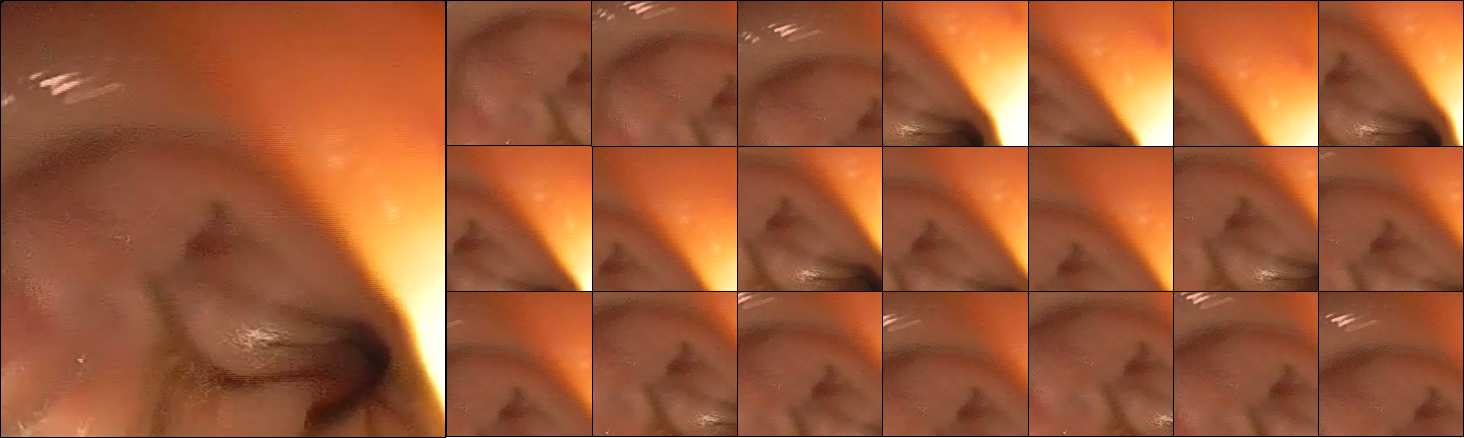
\includegraphics[width=\linewidth]{fine_tuning}
	\caption{A candidate (left) and the patches generated sharing the same label. \cite{zhou}}
	\label{fig:zhou}
\end{figure}

Computer-aided-diagnosis (CAD) systems usually provide a candidate generator, which can quickly produce candidates, including true and false positives, to train classifiers with. The goal is to eleminate as many false positives as possible, while keeping the true ones. Through data augmentation the learner can be made more robust to unforeseen situations. For this numerous patches sharing the same label are generated from the candidate, as can be seen in Figure \ref{fig:zhou}. 

The active selection process of candidates, that produce the largest performance gain when annotated by the user, calls for a measure of the worthiness of a candidate. To achieve this, the entropy and diversity of patches are calculated using the network's predictions for those patches. Entropy is calculated, as expected, as the sum of the negative log-likelihood, whereas diversity captures the summed up differences of the probability values that the network produces for the patches of a specific candidate and label. Intuitively, for a candidate the entropy of all its patches should be high and the diversity low, as the patches are generated from the same candidate and should share the same label. For each candidate a matrix is constructed from these values. The actual active fine-tuning algorithm queries the user for a predefined number, the so-called batch-size, of candidates from a given set. These candidates are selected by their ranking of how much the net will profit from their manual annotation. The network is then fine-tuned with the freshly-acquired data. This operation is repeated with more data from the candidate set until the performance of the network is satisfactory.

The procedure produces good results of 95\% correctly labeled images while using only 5\% of the available dataset for training. Learning from scratch or random selection of next candidates are quickly surpassed in terms of performance. Or to be more precise, the presented method needs around 4 queried labels to achieve the accuracy of the random process at 18 labels or learning from scratch at 22, i.e. saves 75\% or even 80\% annotation cost.

While this makes for an outstanding result, it is rather difficult to map to our problem. The question of how to find such a worthiness measure quickly arises when projecting Zhou et al.'s thinking to pose estimation, as we can't tell how sure a network is when predicting a pose. But it provides a good direction of how to approach active learning.

\quad \textbf{Liu \& Ferrari}

- Scheme for requesting new manually annotated data an retraining
- Convolutional Pose Machine produces heatmaps
- 